\documentclass[12pt]{article}
\usepackage{worksheet-common}

\begin{document}

\worksheettitle{Coulomb's Law Practice}

%============================================================
\partsec{A}{Separation Vectors \& Magnitudes}

\prob Two charges sit on the $x$-axis: $q_1=+3.0\,\mu\text{C}$ at the origin, and $q_2=-5.0\,\mu\text{C}$ at $x=8.0$ cm. Find $\rv{1}{2}$ and $|\rv{1}{2}|$.

\begin{center}
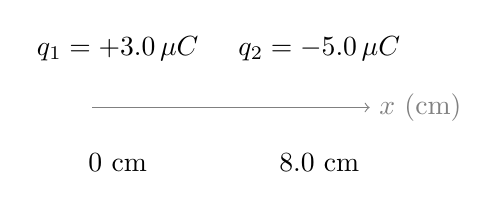
\begin{tikzpicture}[x=0.32cm,y=0.32cm]
\draw[gray,->] (-1,0) -- (10,0) node[right] {$x$ (cm)};
\poscharge{0}{0}{1.3}
\node[above=5pt] at (0,0.9) {$q_1=+3.0\,\mu\text{C}$};
\node[below=5pt] at (0,-0.9) {0 cm};
\negcharge{8}{0}{1.3}
\node[above=5pt] at (8,0.9) {$q_2=-5.0\,\mu\text{C}$};
\node[below=5pt] at (8,-0.9) {8.0 cm};
\end{tikzpicture}
\end{center}

\worksp{lg}

\prob $q_1=+2.0\,\mu\text{C}$ is located at $(1.0\text{ cm},2.0\text{ cm})$. $q_2=-4.0\,\mu\text{C}$ is located at $(5.0\text{ cm},5.0\text{ cm})$. Find $\rv{1}{2}$ and $|\rv{1}{2}|$.

\worksp{lg}

\prob $q_1=+150$ nC sits at the origin. $q_2=-80$ nC sits at $(30\text{ mm},40\text{ mm})$. Find $\rv{1}{2}$ and $|\rv{1}{2}|$, in meters.

\begin{center}
\begin{tikzpicture}[x=0.11cm,y=0.11cm]
\draw[gray,->] (0,0) -- (55,0) node[right] {$x$ (mm)};
\draw[gray,->] (0,0) -- (0,55) node[above] {$y$ (mm)};
\draw[dashed,brown] (0,0) -- (30,40);
\poscharge{0}{0}{3.2}
\node[below left=2pt] at (0,-3.2) {$q_1=+150$ nC};
\negcharge{30}{40}{3.2}
\node[above right=2pt] at (34,42) {$q_2=-80$ nC};
\node[above right=2pt] at (34,35) {$(30,40)$ mm};
\end{tikzpicture}
\end{center}

\worksp{lg}

\prob $q_1=+6.0\times10^{-6}$ C is located at $(1.20\times10^{-2}\text{ m},0)$. $q_2=-2.5\times10^{-6}$ C is located at $(0,1.60\times10^{-2}\text{ m})$. Find $\rv{1}{2}$ and $|\rv{1}{2}|$.

\worksp{lg}

\clearpage
%============================================================
\partsec{B}{Separation Vectors \& Magnitudes --- Multiple Charges}

\prob Three charges: $q_1=+2.0\,\mu\text{C}$ at $(0,0)$, $q_2=-3.0\,\mu\text{C}$ at $(6.0\text{ cm},0)$, $q_3=+5.0\,\mu\text{C}$ at $(0,8.0\text{ cm})$. Find $\rv{1}{2}$ and $\rv{1}{3}$, and their magnitudes.

\begin{center}
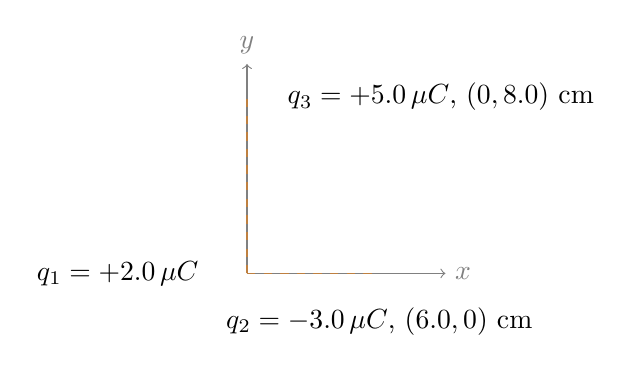
\begin{tikzpicture}[x=0.28cm,y=0.28cm]
\draw[gray,->] (0,0) -- (9,0) node[right] {$x$};
\draw[gray,->] (0,0) -- (0,9.5) node[above] {$y$};
\draw[dashed,brown] (0,0) -- (6,0);
\draw[dashed,brown] (0,0) -- (0,8);
\poscharge{0}{0}{1.2}
\node[left=14pt] at (0,0) {$q_1=+2.0\,\mu\text{C}$};
\negcharge{6}{0}{1.2}
\node[below=4pt] at (6,-0.6) {$q_2=-3.0\,\mu\text{C}$, $(6.0,0)$ cm};
\poscharge{0}{8}{1.2}
\node[right=4pt] at (0.9,8) {$q_3=+5.0\,\mu\text{C}$, $(0,8.0)$ cm};
\end{tikzpicture}
\end{center}

\worksp{xl}

\prob Three charges: $q_1=+100$ nC at $(0,0)$, $q_2=-50$ nC at $(40\text{ mm},0)$, $q_3=+75$ nC at $(24\text{ mm},32\text{ mm})$. Find $\rv{1}{2}$ and $\rv{1}{3}$, and their magnitudes, in meters.

\worksp{xl}

\clearpage

\prob Four charges sit at the corners of a square, 5.0 cm on a side: $q_1=+1.0\,\mu\text{C}$ at $(0,0)$, $q_2=-2.0\,\mu\text{C}$ at $(5.0,0)$ cm, $q_3=+3.0\,\mu\text{C}$ at $(5.0,5.0)$ cm, $q_4=-1.0\,\mu\text{C}$ at $(0,5.0)$ cm. Find $\rv{1}{2}$, $\rv{1}{3}$, and $\rv{1}{4}$, and their magnitudes.

\begin{center}
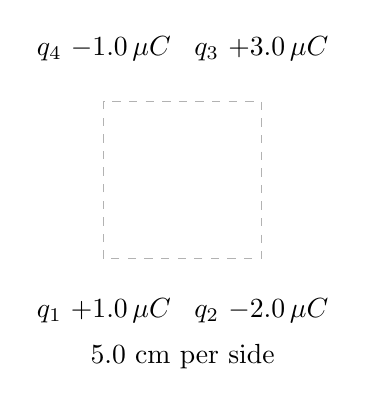
\begin{tikzpicture}[x=0.4cm,y=0.4cm]
\draw[dashed,gray!60] (0,0) rectangle (5,5);
\poscharge{0}{0}{1.0}
\node[below=3pt] at (0,-0.7) {$q_1\ {+1.0\,\mu\text{C}}$};
\negcharge{5}{0}{1.0}
\node[below=3pt] at (5,-0.7) {$q_2\ {-2.0\,\mu\text{C}}$};
\poscharge{5}{5}{1.0}
\node[above=3pt] at (5,5.7) {$q_3\ {+3.0\,\mu\text{C}}$};
\negcharge{0}{5}{1.0}
\node[above=3pt] at (0,5.7) {$q_4\ {-1.0\,\mu\text{C}}$};
\node[below] at (2.5,-2.4) {5.0 cm per side};
\end{tikzpicture}
\end{center}

\worksp{lg}

\prob Four charges: $q_1=+4.0\times10^{-6}$ C at $(2.0,1.0)\times10^{-2}$ m, $q_2=-3.0\times10^{-6}$ C at $(5.0,5.0)\times10^{-2}$ m, $q_3=+2.0\times10^{-6}$ C at $(-1.0,4.0)\times10^{-2}$ m, $q_4=-5.0\times10^{-6}$ C at $(2.0,-3.0)\times10^{-2}$ m. Find $\rv{1}{2}$, $\rv{1}{3}$, and $\rv{1}{4}$, and their magnitudes.

\worksp{xl}

\clearpage
%============================================================
\partsec{C}{Coulomb Force Magnitude}

\textit{Same four setups as Part A. Use Coulomb's law, $F=k|q_1q_2|/r^2$, along with $|\rv{1}{2}|$, to get the magnitude of the force between the charges.}

\prob Same as \probref{1}: $q_1=+3.0\,\mu\text{C}$, $q_2=-5.0\,\mu\text{C}$, separated by 8.0 cm. Find the magnitude of the electric force between them.

\worksp{lg}

\prob Same as \probref{2}: $q_1=+2.0\,\mu\text{C}$ at $(1.0,2.0)$ cm, $q_2=-4.0\,\mu\text{C}$ at $(5.0,5.0)$ cm. Find the magnitude of the force between them.

\worksp{lg}

\prob Same as \probref{3}: $q_1=+150$ nC, $q_2=-80$ nC, at the positions given in \probref{3}. Find the magnitude of the force between them.

\worksp{lg}

\prob Same as \probref{4}: $q_1=+6.0\times10^{-6}$ C, $q_2=-2.5\times10^{-6}$ C, at the positions given in \probref{4}. Find the magnitude of the force between them.

\worksp{lg}

\clearpage
%============================================================
\partsec{D}{Individual Forces}

\textit{Same four setups as Part B. Find the individual force on $q_1$ due to each other charge, one pair at a time --- magnitude and direction. Don't add them together yet. Careful: the force on $q_1$ points along $\vec{r}_{21}=\vec{r}_1-\vec{r}_2=-\vec{r}_{12}$, not $\vec{r}_{12}$ --- you found $\vec{r}_{12}$ in Part B, but the force on $q_1$ needs the vector that points \emph{at} $q_1$, the other way.}

\prob Same as \probref{5}: $q_1=+2.0\,\mu\text{C}$ at $(0,0)$, $q_2=-3.0\,\mu\text{C}$ at $(6.0,0)$ cm, $q_3=+5.0\,\mu\text{C}$ at $(0,8.0)$ cm. Find the force on $q_1$ due to $q_2$ alone, and the force on $q_1$ due to $q_3$ alone.

\worksp{xl}

\prob Same as \probref{6}: $q_1=+100$ nC at $(0,0)$, $q_2=-50$ nC at $(40,0)$ mm, $q_3=+75$ nC at $(24,32)$ mm. Find the force on $q_1$ due to $q_2$ alone, and the force on $q_1$ due to $q_3$ alone.

\worksp{xl}

\clearpage

\prob Same as \probref{7} (the square): $q_1=+1.0\,\mu\text{C}$, $q_2=-2.0\,\mu\text{C}$, $q_3=+3.0\,\mu\text{C}$, $q_4=-1.0\,\mu\text{C}$, 5.0 cm apart along each side. Find the force on $q_1$ due to $q_2$ alone, due to $q_3$ alone, and due to $q_4$ alone.

\worksp{xl}
\vspace{2cm}

\clearpage

\prob Same as \probref{8}: $q_1=+4.0\times10^{-6}$ C, $q_2=-3.0\times10^{-6}$ C, $q_3=+2.0\times10^{-6}$ C, $q_4=-5.0\times10^{-6}$ C, at the positions given in \probref{8}. Find the force on $q_1$ due to $q_2$ alone, due to $q_3$ alone, and due to $q_4$ alone.

\worksp{xl}
\vspace{2cm}

\clearpage
%============================================================
\partsec{E}{Net Force}

\textit{Same four setups one last time. Add the individual forces you found in Part D as vectors to get the net force on $q_1$. Report both the components and the magnitude.}

\prob Using your answers from \probref{13}, find the net force on $q_1$ (magnitude and direction).

\worksp{lg}

\prob Using your answers from \probref{14}, find the net force on $q_1$ (magnitude and direction).

\worksp{lg}

\prob Using your answers from \probref{15}, find the net force on $q_1$ (magnitude and direction).

\worksp{xl}

\clearpage

\prob Using your answers from \probref{16}, find the net force on $q_1$ (magnitude and direction). This is the hardest one on the sheet --- nice work getting here.

\worksp{xl}

%============================================================
\begin{answerkey}
\begin{multicols}{2}

\akpart{Part A --- Separation Vectors}
\akitem{1}{$\rv{1}{2}=(8.0,0)$ cm; $|\rv{1}{2}|=8.0$ cm $=0.080$ m}
\akitem{2}{$\rv{1}{2}=(4.0,3.0)$ cm; $|\rv{1}{2}|=5.0$ cm $=0.050$ m}
\akitem{3}{$\rv{1}{2}=(30,40)$ mm; $|\rv{1}{2}|=50$ mm $=0.050$ m}
\akitem{4}{$\rv{1}{2}=(-1.20,1.60)\times10^{-2}$ m; $|\rv{1}{2}|=2.00\times10^{-2}$ m}

\vspace{2mm}
\akpart{Part B --- Separation Vectors, Multiple Charges}
\akitem{5}{$\rv{1}{2}=(6.0,0)$ cm, $|\rv{1}{2}|=6.0$ cm $\cdot$ $\rv{1}{3}=(0,8.0)$ cm, $|\rv{1}{3}|=8.0$ cm}
\akitem{6}{$\rv{1}{2}=(40,0)$ mm, $|\rv{1}{2}|=40$ mm $\cdot$ $\rv{1}{3}=(24,32)$ mm, $|\rv{1}{3}|=40$ mm}
\akitem{7}{$\rv{1}{2}=(5.0,0)$cm, $|{\cdot}|=5.0$cm $\cdot$ $\rv{1}{3}=(5.0,5.0)$cm, $|{\cdot}|=7.07$cm $\cdot$ $\rv{1}{4}=(0,5.0)$cm, $|{\cdot}|=5.0$cm}
\akitem{8}{$\rv{1}{2}=(3.00,4.00)\times10^{-2}$m, $|{\cdot}|=5.00\times10^{-2}$m $\cdot$ $\rv{1}{3}=(-3.00,3.00)\times10^{-2}$m, $|{\cdot}|=4.24\times10^{-2}$m $\cdot$ $\rv{1}{4}=(0,-4.00)\times10^{-2}$m, $|{\cdot}|=4.00\times10^{-2}$m}

\vspace{2mm}
\akpart{Part C --- Force Magnitude}
\akitem{9}{$F=21.1$ N (attractive)}
\akitem{10}{$F=28.8$ N (attractive)}
\akitem{11}{$F=0.0432$ N $=43.2$ mN (attractive)}
\akitem{12}{$F=337$ N (attractive)}

\vspace{2mm}
\akpart{Part D --- Individual Forces on $q_1$}
\akitem{13}{from $q_2$: $(15.0,0)$ N, 15.0 N $\cdot$ from $q_3$: $(0,-14.0)$ N, 14.0 N}
\akitem{14}{from $q_2$: $(0.0281,0)$ N, 28.1 mN $\cdot$ from $q_3$: $(-0.0253,-0.0337)$ N, 42.1 mN}
\akitem{15}{from $q_2$: $(7.19,0)$ N $\cdot$ from $q_3$: $(-3.81,-3.81)$ N, 5.39 N $\cdot$ from $q_4$: $(0,3.60)$ N}
\akitem{16}{from $q_2$: $(25.9,34.5)$ N, 43.2 N $\cdot$ from $q_3$: $(28.3,-28.3)$ N, 40.0 N $\cdot$ from $q_4$: $(0,-112)$ N}

\vspace{2mm}
\akpart{Part E --- Net Force on $q_1$}
\akitem{17}{$\Fv{}{net}=(15.0,-14.0)$ N; $|\Fv{}{net}|=20.5$ N, $43.2^\circ$ below $+x$}
\akitem{18}{$\Fv{}{net}=(0.00281,-0.0337)$ N; $|\Fv{}{net}|=33.8$ mN, $85.2^\circ$ below $+x$}
\akitem{19}{$\Fv{}{net}=(3.38,-0.218)$ N; $|\Fv{}{net}|=3.38$ N, $3.7^\circ$ below $+x$}
\akitem{20}{$\Fv{}{net}=(54.1,-106)$ N; $|\Fv{}{net}|=119$ N, $63.0^\circ$ below $+x$}

\end{multicols}
\end{answerkey}

\end{document}
